\chapter{Reinforcement Learning}
\section{Overview}
Reinforcement Learning (RL) is a machine learning technique that simulates an agent interacting with the environment. Typical scenario:
    \begin{enumerate}
        \item The agent observes the states from the environment.
        \item The agent performs the action on the environment based on the state observed.
        \item The environment feedback rewards to the agent based on the action performed; the agent will adjust its behavior based on the reward. 
    \end{enumerate}
\begin{figure}[ht]
  \centering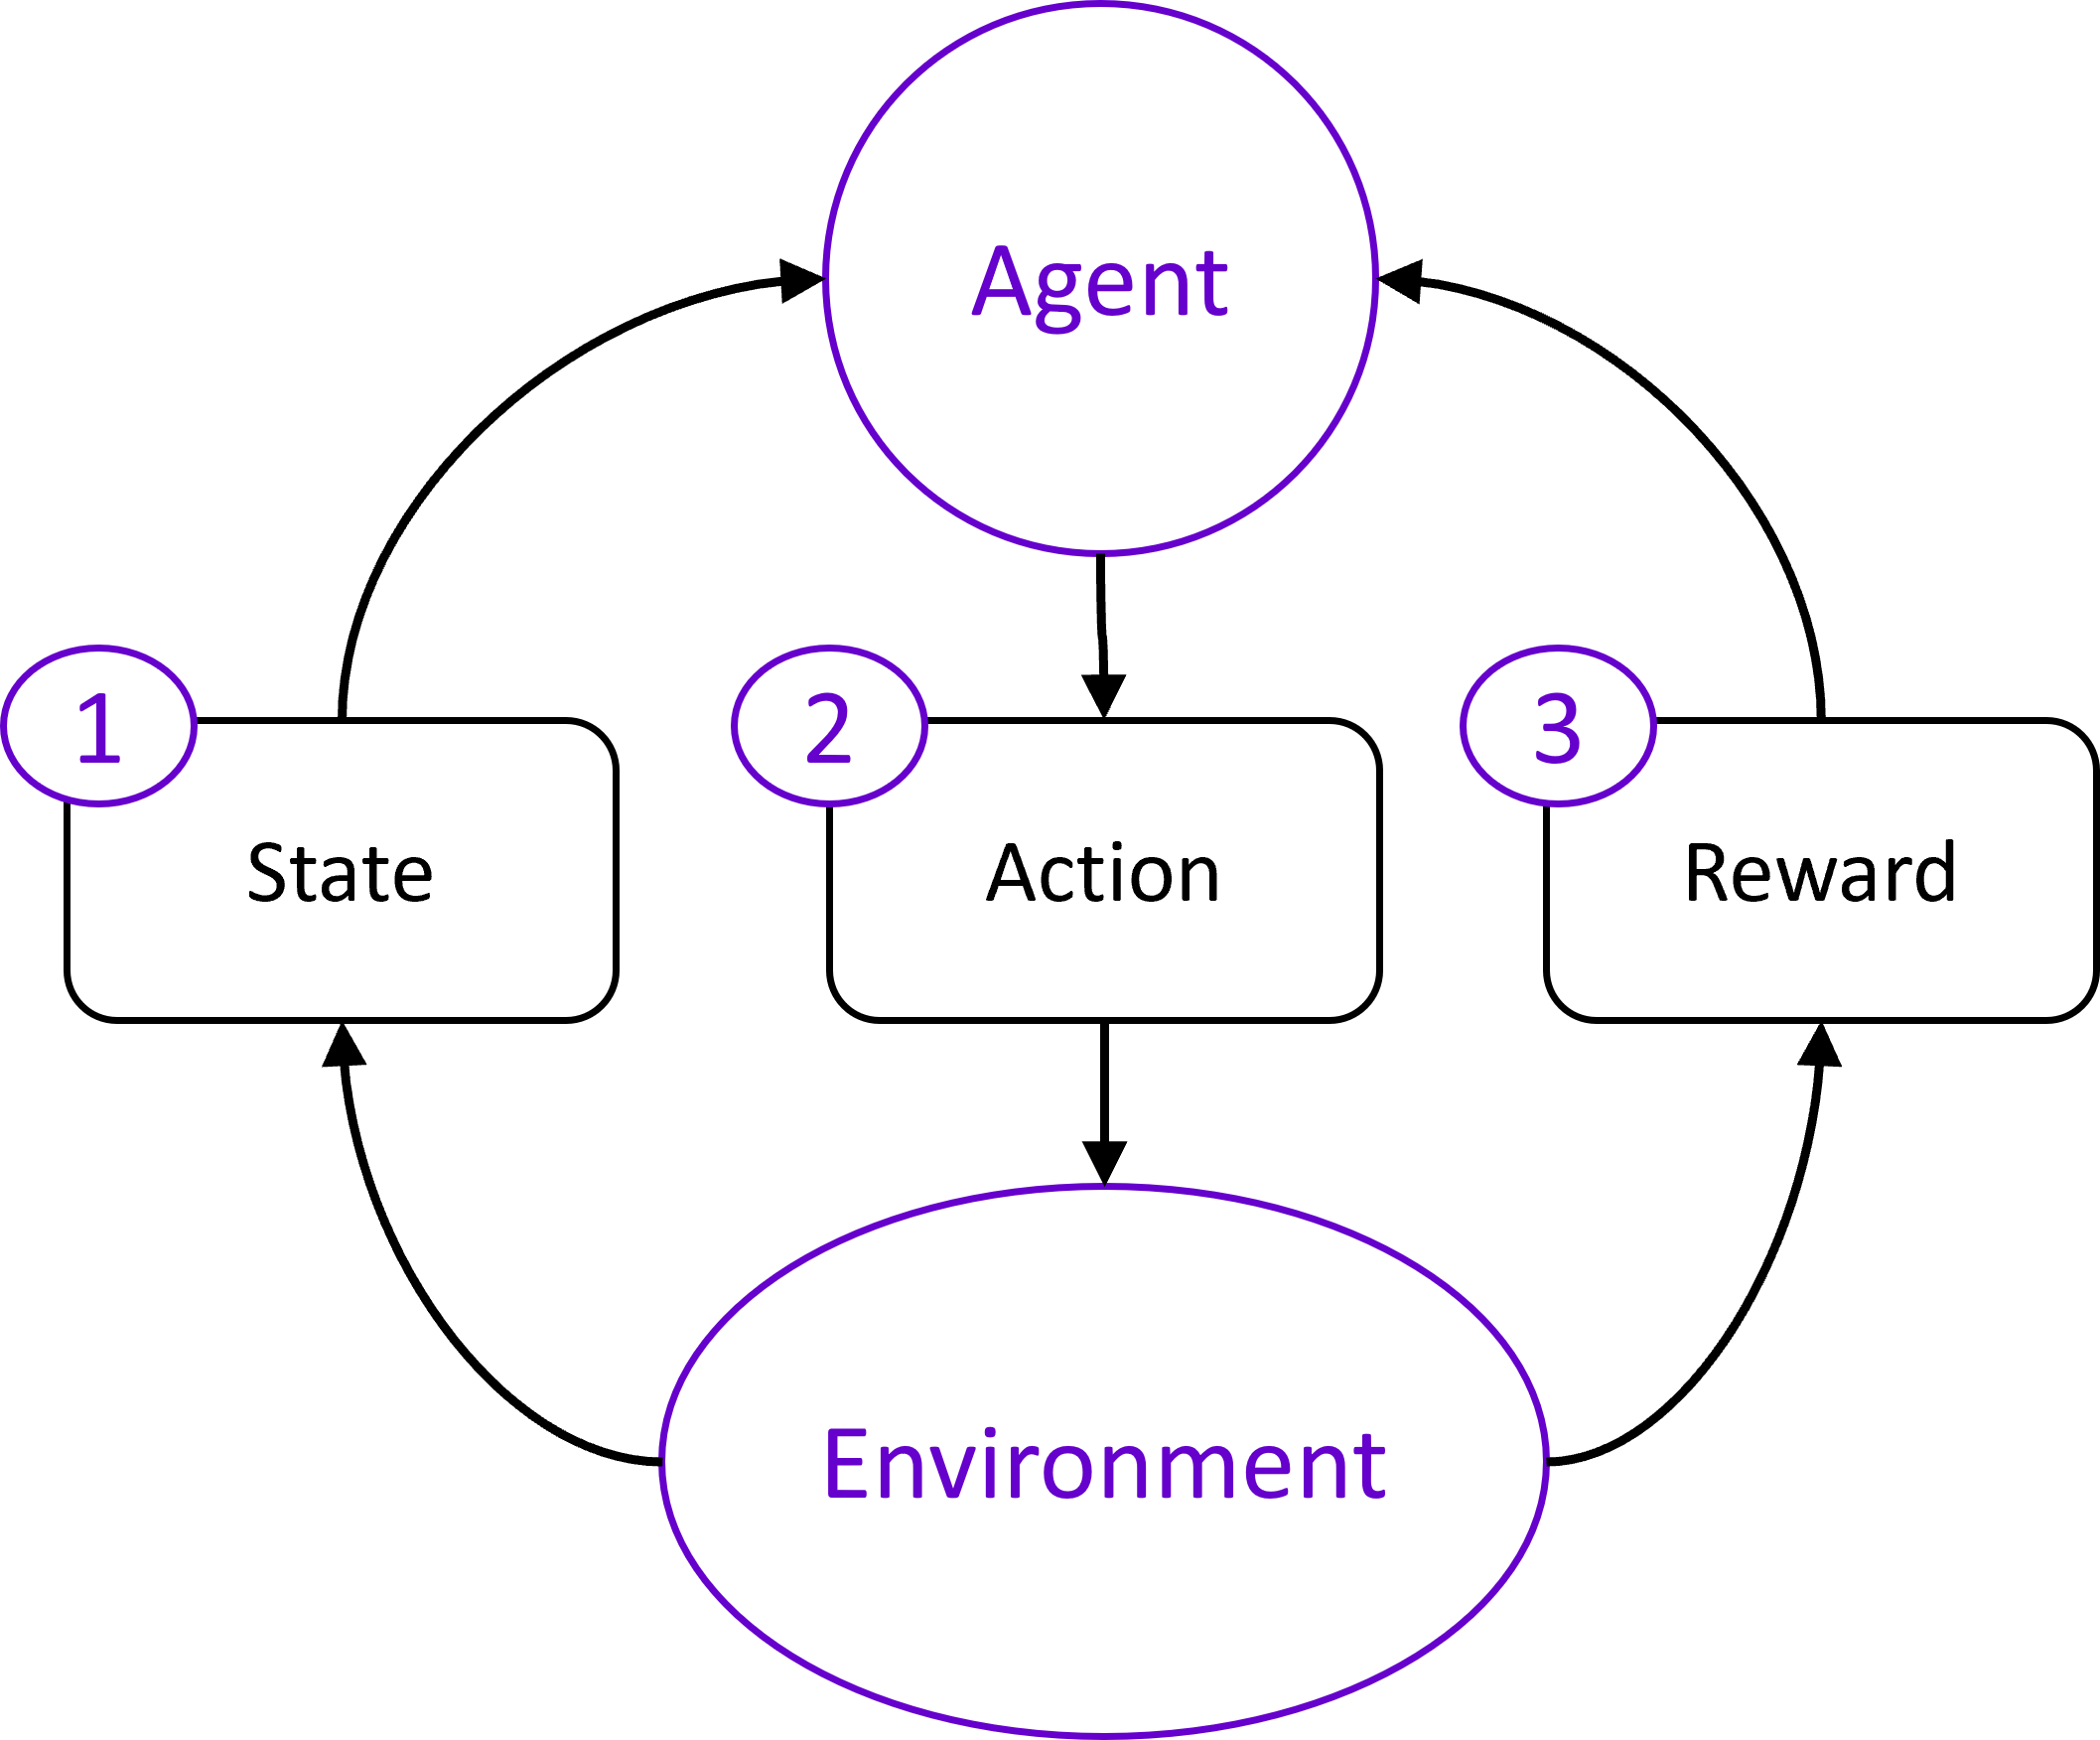
\includegraphics[width=8cm]{images/rl_overview.png}
  \caption [Overview of Reinforcement Learning]
  {Overview of Reinforcement Learning
  }
  \label{fig:rl_overview_diagram}
\end{figure}

\section{Value Function}
The value function is the function to predict the expected reward based on given states and actions. The off-policy algorithm uses value function, e.g., Q learning will have a high sample efficiency with the use of experience replay but will face significant challenges for continuous action spaces since the output space of the value function will be enormous.
\section{Policy}
The policy is the strategy of the agent to perform the action that maximizes the expected reward based on the state.  The typical algorithm uses policy, Policy Gradient can work well with high dimension or continue action spaces. But it has low sample efficiency as it requires a full episode before adjusting the parameters.
\section{Actor Critic}
Actor-Critic uses both the Value Function and the Policy. The actor determines the actions with the policy. The critic uses the value function to criticize the actor's action. Actor-Critic can have high sample efficiency with continuous action spaces.

\section{Deep Reinforcement Learning}
Deep Reinforcement Learning (DRL) combines reinforcement learning (RL) and deep learning. DRL archive remarkable results in many fields, including gaming. We can adapt deep learning networks in many different components of RL, including the value function, or the policy.
\section{Soft Actor-Critic}
Soft Actor-Critic (SAC) is an DRL algorithm that optimizes a stochastic policy in an off-policy way with entropy regularization.
\par
Compare to deterministic policies, stochastic policies provide a stabler result as it favor exploration.
\par 
As a off-policy algorithm, SAC have better sample efficiency with experience replay.
\par
Entropy Regularization balances the exploration-exploitation trade-off as the algorithm favors exploration when the entropy is high initially and becomes more deterministic when entropy is low to increase exploitation.